%
% This docuement is based on the Insight Journal Template.
% https://github.com/InsightSoftwareConsortium/InsightJournalTemplate/tree/ModularTemplate
% 4555fc04b105b11f06dc302b76bf09c27e50727d

\documentclass{InsightArticle}

\usepackage[dvips]{graphicx}
%  hyperref should be the last package to be loaded.
\usepackage[dvips,
bookmarks,
bookmarksopen,
float,
backref,
colorlinks,linkcolor={blue},citecolor={blue},urlcolor={blue},
]{hyperref}

\title{BinShrink: A multi-resolution filter with cache efficient averaging. }

\newcommand{\IJhandlerIDnumber}{0}

\release{0.00}

% At minimum, give your name and an email address.  You can include a
% snail-mail address if you like.
\author{Bradley C. Lowekamp$^{1}$ and David T. Chen$^{1}$}
\authoraddress{$^{1}$National Library Of Medicine}

\begin{document}

%
% Add hyperlink to the web location and license of the paper.
% The argument of this command is the handler identifier given
% by the Insight Journal to this paper.
% 
\IJhandlefooter{\IJhandlerIDnumber}


\ifpdf
\else
   %
   % Commands for including Graphics when using latex
   % 
   \DeclareGraphicsExtensions{.eps,.jpg,.gif,.tiff,.bmp,.png}
   \DeclareGraphicsRule{.jpg}{eps}{.jpg.bb}{`convert #1 eps:-}
   \DeclareGraphicsRule{.gif}{eps}{.gif.bb}{`convert #1 eps:-}
   \DeclareGraphicsRule{.tiff}{eps}{.tiff.bb}{`convert #1 eps:-}
   \DeclareGraphicsRule{.bmp}{eps}{.bmp.bb}{`convert #1 eps:-}
   \DeclareGraphicsRule{.png}{eps}{.png.bb}{`convert #1 eps:-}
\fi


\maketitle


\ifhtml
\chapter*{Front Matter\label{front}}
\fi

% The abstract should be a paragraph or two long, and describe the
% scope of the document.
\begin{abstract}
\noindent
We present a new filter for the Insight Toolkit (ITK), to reduce the
resolution of an image by integer factor while averging call
\textit{BinShrink}. This filter provides a new levels of performance to
ITK for reducing resolution and noise present in an image. The filter
support streaming, multi-threading and most of ITK's pixel types
including scalars, \textit{Vector}s,
\textit{SymmetricSecondRankTensor}s, and \textit{RGBPixel}s.

\end{abstract}

\IJhandlenote{\IJhandlerIDnumber}

\tableofcontents

Using filters from the Insight Toolkit, we develop an algorithm for detecting
and tracking thje movement of solar spots. As it is widely known, celestial
objects such as the sun are ethereal and perfect, and therefore can not harbor
artifacts such as spots. However, observations performed with our open source
telescope have revealed the presence of such spots. The spots seems to continuously change positions on the solar surface. 


% don't like
This ``binning'' algorithm is commonly used in processing of high
resolution electron microscopy image. It's available in such packages
as The Boulder Laboratory for 3-D Electron Microscopy of Cell's
IMOD\cite{IMOD}, \cite{bsoft2007}. 
Multi-resolution

why is this fitlter useful?


This document describes a new algorithm not currently in
itk\cite{ITKSoftwareGuide}. 

\section{Implementation}

Algorithm

Features

\subsection{Geometry}


\begin{figure}
  \centering
  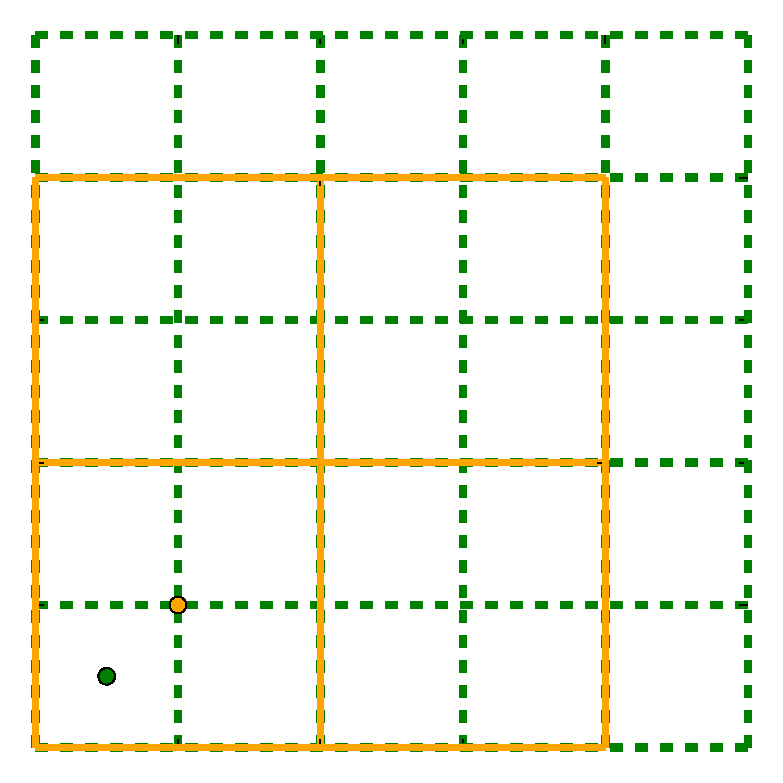
\includegraphics[width=0.8\linewidth]{images/pixelgrid}
  \itkcaption{Grid Geometry}
  \label{fig:PixelGrid}
\end{figure}

\subsection{Optimization}
Optimization 


\section{Results}

To view the output of this filter we have used a synthetic function
created by Marschner and Lobb\cite{MarschnerL94}, along with additive
noise to create volume. This function has been used previously to
evaluate volume rendering reconstruction filters. We have rendered
into a 128 pixel cubic volume such that the majority of the frequencies in
the function are sampled just above 4 times the Nyquist frequency. This makes
for challenging theoretical data set when the shrinking factor is also
4.

The code used to generate these images was written in Python with
SimpleITK. The original Marshner-Lobb volume was normalized with the 
\textit{Normalize} filter so that the volume had a mean
of 0 and a standard deviation of 1. Then Gaussian distributed random
noise was added with a 0 mean and a sigma to achieve the targeted
signal to noise ratio. After the shrinking operation was performed,
the volume was again normalized for contrast. Then the center slice
was extracted and tiles. Lastly it was colorized by the
\textit{ScalarToRGBColormap} filter\cite{Tustison2009}.

We have composed a study for \textit{BinShrink} filter by varying the
signal to noise ratio and shrinking by 2 and 4 (See figure
\ref{fig:BinShrinkComparison}). Also for comparison we have used the
\textit{SmoothingRecusiveGaissian} filter in conjunction with the
\textit{Shrink} filter where \textit{sigma} used to define the
smoothing Gaussian kernel is 0.7 times the shrink factor. 

\begin{figure}
  \centering
  
\includegraphics[width=0.4\linewidth]{images/binshrink_hot.png}
  \caption[Registration Framework Components]{The basic components of the
    registration framework are two input images, a transform, a metric, an
    interpolator and an optimizer.}
  \label{fig:BinShrinkComparison}
\end{figure}

\begin{figure}
  \centering
  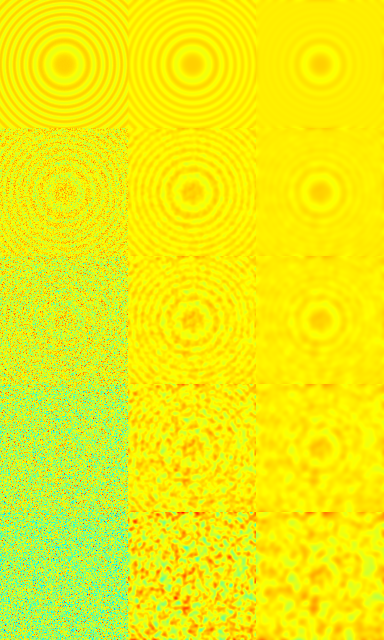
\includegraphics[width=0.4\linewidth]{images/gaussianshrink_hot.png}
  \caption[Registration Framework Components]{The basic components of the
    registration framework are two input images, a transform, a metric, an
    interpolator and an optimizer.}
  \label{fig:GaussianShrinkComparison}
\end{figure}

\subsection{Performance}

To analyze the performance of our bin shrink methods we compare them
against similar process which can be done in ITK with two filters.

By running a \textit{Mean} filter followed by a \textit{Shrink} filter a
close approximation to \textit{BinShrink} can be done. The
\textit{Mean} filter runs a average for each input pixel's
neighborhood in a brute force fashion. This wastes computation on input
pixel that are just dropped by the \textit{Shrink} filter.

Using a Gaussian kernel to reduce aliasing is an alternative to the box
kernel implicitly used with the \textit{BinShrink} filter. This can be
done with constant time independent of the size of the Gaussian with
the \textit{SmoothingRecusiveGaussian} filter.


We generated a Gaussian distributed 256 pixel cubic image for
performance evaluation. Utilizing SimpleITK and Python's
\textit{timeit} module, we report the median of 3 runs for each
algorithm across varying shrink factors (See Figure
\ref{fig:ShrinkPerformance}). The system... As expected the \textit{Mean} approach
suffers from exponential cost while the
\textit{SmoothingRecursiveGaussian} method remains constant. While the
\textit{BinShrink2} implementation only touches each input pixel once,
it also suffers from exponential growth likely due to it's memory
access pattern being inefficient and not cache coherent. On the other
hand the \textit{BinShrink} implementation execution time decreases as
the shrink factor increases.

\begin{figure}
  \centering
  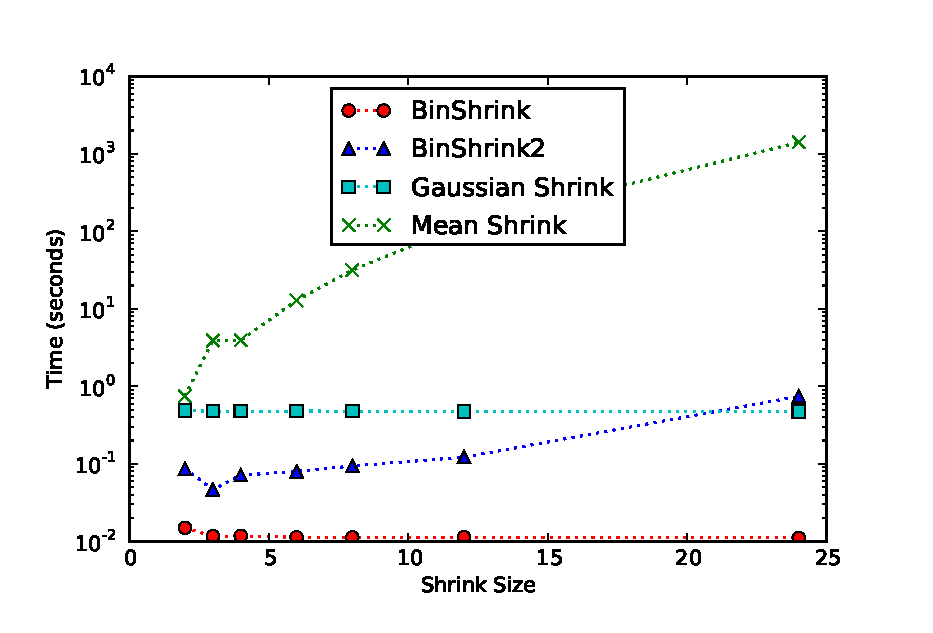
\includegraphics[width=0.8\linewidth]{images/shrink_time}
  \itkcaption{Performance}
  \label{fig:ShrinkPerformance}
\end{figure}

\section{Conclusion}




%  Example 



To support shape-guidance, the generic level set equation
(Eqn(~\ref{eqn:ShapeInfluenceTerm})) is extended to incorporate a shape guidance
term:

\begin{equation}
\label{eqn:ShapeInfluenceTerm}
\xi \left(\psi^{*}(\mathbf{x}) - \psi(\mathbf{x})\right)
\end{equation}




%%%%%%%%%%%%%%%%%%%%%%%%%%%%%%%%%%%%%%%%%
%
%  Insert the bibliography using BibTeX
%
%%%%%%%%%%%%%%%%%%%%%%%%%%%%%%%%%%%%%%%%%

\bibliographystyle{plain}
\bibliography{BinShrink}


\end{document}

